\documentclass{article}

\usepackage{tikz}
%\usepackage{rotating}
 

\begin{document}
%\begin{turn}{90}
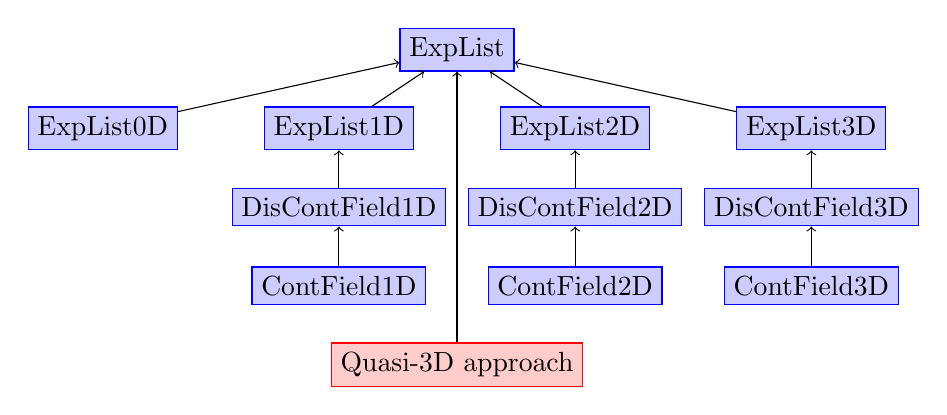
\begin{tikzpicture}[outline/.style={draw=#1,fill=#1!20}]

%NODES

% level (1) 
\node [outline=blue] (ExpList)                                   at (4.5,0)          {ExpList};
% level (2) y = -2
\node [outline=blue] (ExpList0D)                              at (0,-1)        {ExpList0D};
\node [outline=blue] (ExpList1D)                              at (3,-1)        {ExpList1D};
\node [outline=blue] (ExpList2D)                              at (6,-1)        {ExpList2D};
\node [outline=blue] (ExpList3D)                              at (9,-1)        {ExpList3D};
% level (4) 
\node [outline=blue] (DisContField1D)                    at (3,-2)         {DisContField1D};
\node [outline=blue] (DisContField2D)                    at (6,-2)         {DisContField2D};
\node [outline=blue] (DisContField3D)                    at (9,-2)         {DisContField3D};
% level (5) y 
\node [outline=blue] (ContField1D)                    at (3,-3)         {ContField1D};
\node [outline=blue] (ContField2D)                    at (6,-3)         {ContField2D};
\node [outline=blue] (ContField3D)                    at (9,-3)         {ContField3D};
% level (3) y = -3.5
\node [outline=red] (Quasi-3D approach)                         at (4.5,-4)           {Quasi-3D approach};
%CONNECTIONS

\path[<-]  (ExpList)      edge (ExpList0D)
                 (ExpList)      edge (ExpList1D)
                 (ExpList)      edge (ExpList2D)
                 (ExpList)      edge (ExpList3D)
                 (ExpList)      edge (Quasi-3D approach)
                
                 (ExpList1D) edge (DisContField1D)
                 (ExpList2D) edge (DisContField2D)
                 (ExpList3D) edge (DisContField3D)
                 
                 (DisContField1D)  edge (ContField1D)
                 (DisContField2D)  edge (ContField2D)
                 (DisContField3D)  edge (ContField3D);
\end{tikzpicture}
%\end{turn}

\end{document}